\documentclass{lms}
\usepackage[utf8]{inputenc}
\usepackage[american]{babel}
\usepackage[T1]{fontenc}
\usepackage{amssymb,amsmath,amsfonts}
\usepackage{algorithmic}
\usepackage{algorithm}
\usepackage{tikz}
\usepackage{nicefrac}
\usepackage{hyperref}
\usepackage{unicode}
\usepackage{stmaryrd}
 
\newcommand{\todo}[1]{{\color{red}TODO: #1}}
\def\snote#1{\marginpar{{\color{blue}%
%   \rlap{\hskip 50pt \vrule height 1pt width 20pt}%
%   \leavevmode\kern 7pt \vbox{\hsize 56pt\kern -8pt
  \fontsize{7pt}{8pt}\selectfont #1\par}}}


%\theoremstyle{plain}
\newtheorem{thm}{Theorem}[section]
\newtheorem{lem}[thm]{Lemma}
\newtheorem{cor}[thm]{Corollary}
\newtheorem{prop}[thm]{Proposition}

\newnumbered{defi}[thm]{Definition}
\newnumbered{rem}{Remark}
\newnumbered{exe}{Example}
\newnumbered{prob}{Problem}

\def\mat#1{\begin{pmatrix}#1\end{pmatrix}}
\def\smat#1{{\def\arraystretch{.7}\mat{#1}}}
\def\pa#1{\left(#1\right)}
\def\acco#1{\left\{#1\right\}}
\def\bcro#1{\left\llbracket#1\right\rrbracket}
\def\chev#1{\left\langle#1\right\rangle}
% pour les coûts des opérations M, F etc. (?)
\def\cout#1{\mathsf{#1}}
% let's decide on one!
\let\leq\leqslant \let\geq\geqslant

\newcommand{\F}{\mathbb{F}}
\newcommand{\Q}{\mathbb{Q}}
\newcommand{\C}{\mathbb{C}}
\newcommand{\tildO}{\tilde{O}}
\newcommand{\MM}{\cout{M}}
\newcommand{\FF}{\cout{F}}
\newcommand{\RR}{\cout{R}}
\DeclareMathOperator{\loglog}{loglog}

\def\algorithmicrequire{\textbf{Input:}}
\def\algorithmicensure{\textbf{Output:}}

\makeatletter
\def\full@line{8pt}
\def\doublefull@line{12pt}
% \def\@nprf{% nprf environment modified OT 12/11/02
%   \list{}{\topsep 8pt \leftmargin 0pt
%   \itemindent\parindent \labelsep .5em 
%   \listparindent\parindent
%   \settowidth\labelwidth{{\normalfont\rmfamily(iii)}}}%
%   \item{\normalfont\itshape\proofname.}\advance\itemindent\labelsep%
%   \advance\itemindent\labelwidth%
%   \hskip 1em\normalfont\rmfamily\ignorespaces}
\makeatother


% Colors after XKCD color name survey
\definecolor{purple}{rgb}{.49,.11,.61}
\definecolor{green}{rgb}{.08,.69,.10}
\definecolor{blue}{rgb}{.01,.26,.87}
\definecolor{pink}{rgb}{1,.5,.75}
\definecolor{brown}{rgb}{.39,.21,.00}
\definecolor{red}{rgb}{.89,0,0}
\definecolor{lightblue}{rgb}{.58,.81,.98} 
\definecolor{teal}{rgb}{0,.57,.52}
\definecolor{orange}{rgb}{.97,.45,.02}
\definecolor{lightgreen}{rgb}{.53,.99,.01}
\definecolor{magenta}{rgb}{.76,0,.47}
\hypersetup{colorlinks,linkcolor={red!70!black},
  citecolor={green!70!black},urlcolor={blue!70!black}}

\title[Explicit isogenies in any characteristic]{Explicit isogenies in quadratic time in any characteristic}
\author{Cyril Hugounenq}

\classno{11Y40 (primary), 11G20, 14H52 (secondary)}

\extraline{This work was partially supported by the
  \href{http://www.digiteo.fr/}{DIGITEO} grant 2013-0531D (ARGC).}

\begin{document}
\maketitle

\begin{abstract}
The problem we will consider here is the computation of an isogeny between two elliptics curves with the knowledge of the domain and the codomain of the isogeny and it's degree $r$. Couveignes's algorithm is an algorithm which solves this problem in $O(r^2)$ operations using the $p$-torsion. We want to extend the method used by Couveignes  We try to adapt his method here to the case of the $2$ torsion and more generally to the $\ell$ torsion, thus we propose an alternative for medium characteristic with this algorithm.
\end{abstract}

% \section*{Proposed notation}

% This section is for internal reference only: erase after the paper has
% stabilized.

% \begin{itemize}
% \item $\mathbb{F}_q$ is the field we are working on
% \item $\ell$ is for the $\ell$ torsion we are working on
% \item $r$ is the degree of the isogeny we want to compute
% \item $k$ is the integer such that $\ell^{2k}>4r+1$
% \item we thus work with a tower which has for top level $F_{q^{\ell^k}}$
% \item $E$ is for ordinary elliptic curves defined over the finite field $\mathbb{F}_q$
% \item $\mathcal{O}$ (resp. $\mathcal{O}_x$) is the notation for the endomorphism ring associated (up to isomorphism) to $E$ (resp. $E_x$)
% \item $K$ is the notation for the imaginary quadratic field in which $\mathcal{O}$ is defined
% \item $d_K$ is the negative integer such that $K=\mathbb{Z}[d_K]$  
% \end{itemize}

%%%%%%%%%%%%%%%

\section{Introduction}
\label{sec:introduction}

Isogenies are non-zero morphisms of elliptic curves, that is,
non-constant rational maps preserving the point at infinity. They are
also algebraic group morphisms. Isogeny computations play a central
role in the algorithmic theory of elliptic curves. They are notably
used to speed up Schoof's point counting
algorithm\cite{schoof85,atkin88,elkies92,schoof95,elkies98}. They are
also widely applied in cryptography, where they are used to speed up
point multiplication~\cite{gallant+lambert+vanstone01,birkner+sica11},
to perform cryptanalysis~\cite{mauer+menezes+teske01}, and to
construct new
cryptosystems~\cite{teske06,charles+lauter+goren09,Stol,defeo+jao+plut12,jao+soukharev2014-signatures}.

The \emph{degree} of an isogeny is its degree as a rational map. If an
isogeny has degree $r$, we call it an $r$-isogeny, and we say that two
elliptic curves are $r$-isogenous if there exists an $r$-isogeny
relating them. Accordingly, we say that two field elements $j$ and
$j'$ are $r$-isogenous if there exist $r$-isogenous elliptic curves
$E$ and $E'$ such that $j(E)=j$ and $j(E')=j'$. The
\emph{explicit isogeny} problem has many incarnations. In this paper,
we are interested in the variant defined below.

\begin{prob}[(Explicit isogeny problem)] \label{prob:isogeny-problem}
  Given two $j$-invariants $j$ and $j'$, and a positive integer
  $r$, determine if they are $r$-isogenous. In that case, compute
  curves $E$, $E'$ with $j(E)=j$ and $j(E')=j'$, and the
  kernel of an $r$-isogeny $ψ:E\to E'$.
\end{prob}

Once the kernel of the isogeny is computed, the rational maps
associated to it can be computed in optimal time using Velu's
formulas~\cite{velu71}.

This paper focuses on the explicit isogeny problem for \emph{ordinary}
elliptic curves over finite fields. A famous theorem by Tate states
that two curves are isogenous over a finite field if and only if they
have the same cardinality over that field. The explicit isogeny
problem stated here appears naturally in the Schoof-Elkies-Atkin point
counting algorithm (SEA). There, $E$ is the curve of which we want to
compute the cardinality, and $E'$ is an $r$-isogenous curve, with $r$
a prime of size approximately $\log\#E$. For this reason, the explicit
isogeny problem is customarily solved without prior knowledge of the
cardinality of $E$. We will abide by this convention here.

A good measure of the computational difficulty of the problem is given
by the isogeny degree $r$. Indeed the output is represented by
$O(r)$ base field elements, hence an asymptotically optimal algorithm
would solve the problem using $O(r)$ field operations. Many algorithms
have been suggested over the years to solve the explicit isogeny
problem. Early algorithms were due to Atkin~\cite{atkin91} and
Charlap, Coley and
Robbins~\cite{charlap1991enumeration}. Elkies'~\cite{elkies92,elkies98,Bostan}
was the first algorithm targeted to finite fields (of large enough
characteristic). Assuming $r$ is prime, its complexity is dominated by
the computation of the modular polynomial $\Phi_r$, which is an object
of (binary) size $O(r^3\log r)$. Later Bröker, Lauter and
Sutherland~\cite{sutherland10:modpol} optimized the modular polynomial
computation in the context of the SEA
algorithm. Finally Lercier and Sirvent\cite{lercier+sirvent08,1602.00244}
generalized Elkies' algorithm to work in any characteristic. Despite
these advances, the overall cost of Elkies' algorithm and its
variants is still at least cubic in $r$.

Another line of work to solve the explicit isogeny problem was
initiated by Couveignes~\cite{couveignes94,couveignes96,couveignes00},
and later improved by De Feo and Schost~\cite{df10,df+schost12}. These
algorithms use an interpolation approach combined with ad-hoc
constructions for towers of finite fields of characteristic $p$. Their
complexity is quasi-quadratic in $r$, but exponential in $\log p$,
hence they are only practical for very small characteristic.

In this paper we present a variant of Couveignes' algorithm with
complexity polynomial in $\log p$ and quasi-quadratic in $r$. Together
with the Lercier-Sirvent algorithm, they are the only polynomial-time
isogeny computation algorithms working in any characteristic, hence
they are especially relevant for counting points in \emph{medium}
characteristic (i.e., counting points over $\F_{p^n}$, when
$n\gg p/\log p$).

Note that, although Couveignes-type algorithms do not make use of the
modular polynomial $\Phi_r$, its computation is still necessary in the
context of the SEA algorithm. Thus our new algorithm does not improve
the state of the art on point counting \todo{but maybe benchmarks are
  going to show that, at least in practice, we sometimes beat
  Lercier-Sirvent?}. It gives, however, an effective algorithm for
solving the explicit isogeny problem, with potential applications in
other contexts, e.g., cryptography.

\subsection{Notations}

Throughout this paper: $r$~is a positive integer, $p$~an odd prime,
$q$~a power of $p$, and $\mathbb F_q$ is the finite field with
$q$~elements. $E$ ~is an ordinary elliptic curve over~$\mathbb F_q$,
its group of $n$-torsion points is denoted by~$E[n]$, its
$q$-Frobenius automorphism by~$π$.  The endomorphism ring of $E$ is
denoted by~$\mathcal O$, with~$K = \mathcal O ⊗ ℚ$ the corresponding
number field, $\mathcal O_K$ is its maximal order, and $d_K$~the
discriminant of~$\mathcal O_K$.
For a prime~$ℓ$ different from~$p$ and not dividing~$r$,
we denote by~$E[ℓ^n]$ the group of $ℓ^n$-torsion points of~$E$,
$E[ℓ^{∞}] = \varinjlim E[ℓ^n]$ the reunion of all $E[ℓ^n]$,
and $T_ℓ(E) = \varprojlim E[ℓ^n]$ the $ℓ$-adic Tate module~\cite[III.7]{Sil},
which is free of rank~two over~$ℤ_ℓ$.
The factorization of the characteristic polynomial of~$π$
in~$ℤ_ℓ$ is determined by the Kronecker symbol~$(d_K/ℓ)$.
If $(d_K/ℓ) = +1$ then we also define $λ,μ$ as
the eigenvalues of~$π$ in~$ℤ_ℓ$ and write~$h = v_ℓ(λ - μ)$,
where $v_ℓ$ is the $ℓ$-adic valuation.

We measure all computational complexities in terms of operations in
$\mathbb{F}_q$, we use the Landau notation $O()$ to express
asymptotic complexities, and the notation $\tildO()$ to neglect
polylogarithmic factors.  We let $\MM(n)$ be a function such that
polynomials in $\F_q[X]$ of degree less than $n$ can be multiplied
using $\MM(n)$ operations in $\F_q$, under the assumptions
of~\cite[Ch.~8.3]{vzGG}. Using FFT multiplication, one can take
$\MM(n)∈ O(n\log n\loglog n)$.

\subsection{Towers of finite fields}
\label{sub:towers}

The algorithms presented next operate on elements defined in finite
extensions of $\F_q$. Specifically, we define a \emph{tower} of finite
fields $\F_q=F₀⊂F₁⊂\cdots⊂F_k$ with $\ell$ dividing $\#F_1-1$, $[F₁:F₀]$
dividing $ℓ-1$, and $[F_{i+1}:F_i]∈\{1,ℓ\}$ for any $i>0$. For $ℓ=2$,
we build upon the work of Doliskani and Schost~\cite{DoSc12}. For
general $ℓ$ we use towers of Kummer extensions in a way similar
to~\cite[\S~2]{DeDoSc13}.  Both constructions represent elements of
$F_i$ as univariate polynomials with coefficients in $\F_q$, thus
basic arithmetic operations can be performed with classic modular
polynomial arithmetic. While constructing the tower, we also enforce
special relations between the generators of each level, so that moving
elements up and down the tower, and testing membership, can be done at
negligible cost.

We briefly sketch the construction for odd $\ell$. Let $d_1=[F₁:F₀]$,
we first look for a primitive polynomial $P_1∈\F_q[x]$ of degree
$d_0$. There are many probabilistic algorithms to compute $P_1$ in
time polynomial in $\ell$ and $\log q$; since their cost does not
depend on the height $k$ of the tower, we neglect it. Then, the image
$x₁$ of $x$ in $F_1=\F_q[x]/P₁(x)$ is an element of multiplicative
order $\#F₁-1$, and in particular it is a non $ℓ$-adic residue. Let
now $e_i=[F_i:F_1]$, we define $F_i$ as $\F_q[x]/P_1(x^{e_i})$, which
does not require any algebraic computation. Using this representation,
elements of $F_i$ can be expressed as elements of a higher level, and
reciprocally, by a simple rearrangement of the coefficients. The
construction for $\ell=2$ is similar, but Doliskani and
Schost~\cite{DoSc12} enrich it with several non-trivial algorithms for
advanced arithmetic operations such as field traces and square roots.

Summarizing, the following computations can be performed at the same
asymptotic cost for any $ℓ$:
\begin{itemize}
\item basic arithmetic operations (addition, multiplication) in $F_i$,
  using $O(\MM(ℓ^i))$ operations;
\item inversion in $F_i$ using $O(i\MM(ℓ^i)\logℓ)$
  operations\footnote{When $ℓ=2$, a factor of $i$ can be saved
    here~\cite{DoSc12}, but we will disregard this optimization for
    simplicity.};
\item mapping elements from $F_{i-1}$ to $F_i$ and \emph{vice versa}
  at no arithmetic cost;
\item multiplication and Euclidean division of polynomials of degree
  at most $d$ in $F_i[x]$ using $O(\MM(dℓ^i))$ operations;
\item computing a $q^{\ell^{j}}$ power in $F_i$ using $O(\ell^i+\log(q))$ operations, the case $\ell=2$ was a result from Doliskani and Schost, the case $\ell \neq 2$ is proved in \ref{lemma:frob-ell} using a generalisation of the case $\ell=2$.
\end{itemize}

For one fundamental operations, we only have an efficient algorithm in
the case $ℓ=2$, hence we introduce the following notations:
\begin{itemize}
%\item $\FF(i,j)$ is the cost of computing a $q^{ℓ^j}$-th power in
%  $F_i$;
\item $\RR(i)$ is the cost of finding a root of a polynomial of degree
  $ℓ$ in $F_i[x]$.
\end{itemize}
For $\ell=2$, Doliskani and Schost show that %$\FF(i,j)=O(ℓ^i+\log q)$, and
 $\RR(i)=O(\MM(ℓ^i)\log(ℓ^iq))$. For general $ℓ$, we have
%$F(i,j)=O(ℓ^{i+j}\log q)$ using a naive algorithm, and
$\RR(i)=O(ℓ^i\MM(ℓ^{i+1})\logℓ\log(ℓq))$ using the variant of the
Cantor-Zassenhaus algorithm described in \cite[\S~14.5]{vzGG}, or
$\RR(i)=O\bigl((ℓ^{i(ω+1)/2}+\MM(ℓ^{i+1}\log q))i\logℓ\bigr)$
using~\cite{kaltofen+shoup97}.


\subsection{Couveignes' algorithm}
\label{sec:couv-algor}

Couveignes' isogeny algorithm takes as input two \emph{ordinary}
elliptic curves $E$ and $E'$, and a positive integer $r$ not
divisible by $p$, and returns, if it exists, the kernel of an
$r$-isogeny $ψ:E\to E'$. It is based on the observation that the
isogeny $ψ$ must put $E[p^k]$ in bijection with $E'[p^k]$, in a way
that is compatible with their group structure. It proceeds in three
steps:
\begin{enumerate}
\item\label{alg:orig-couveignes:tower} Compute generators $P,P'$ of
  $E[p^k]$ and $E'[p^k]$ respectively, for $k$ large enough;
\item\label{alg:orig-couveignes:interp} Compute the interpolation
  polynomial $\mathcal{A}$ \todo{(verify that notation is consistent
    with Sec.5)} sending $x(P)$ to $x(P')$, and the abscissas of
  their scalar multiples accordingly;
\item\label{alg:orig-couveignes:rational} Deduce a rational fraction
  congruent to $\mathcal{A}$ modulo $E[p^k]$, and verify that it
  defines an isogeny of degree $r$. If it does, return it, otherwise
  replace $P'$ with a scalar multiple of itself and go back to
  Step~\ref{alg:orig-couveignes:interp}.
\end{enumerate}

For this algorithm to succeed, enough interpolation points are
required. Given that the isogeny $ψ$ is defined by a rational fraction
of degree $(r,r-1)$, it is necessary that $p^k∈O(r)$. However, most of
the time, those points are not going to be defined in the base field
$\F_q$, thus Couveignes' algorithm must be based on efficient
algorithms to construct and compute in towers of extensions of finite
fields. Indeed, Couveignes and his successors go at great length in
studying the arithmetic of \emph{Artin-Schreier
  towers}~\cite{couveignes00,df+schost12}, and the adaptation of the
fast interpolation algorithm to that setting~\cite{df10}.  Using these
highly specialized constructions,
Steps~\ref{alg:orig-couveignes:tower}
and~\ref{alg:orig-couveignes:interp} are both executed in quasi-linear
time $\tildO(p^{k+O(1)})=\tildO(rp^{O(1)})$. However the last step
only succeeds for one pair of torsion points $P,P'$, in general, thus
$O(r)$ trials are expected on average.

Hence, the overall complexity of Couveignes' algorithm is
$\tildO(r²p^{O(1)})$, i.e., quadratic in $r^2$, but exponential in
$\log p$. Although the exponent of $\log p$ is relatively small, Couveignes
algorithm quickly becomes impractical as $p$ grows.

\subsection{Our contributions}

In this paper we
introduce a variant of Couveignes' algorithm with the same quadratic
complexity in $r$, and \textbf{no exponential dependency in $\log p$}.

The bottom line of our algorithm is elementary: replace $E[p^k]$ in
the algorithm with $E[ℓ^k]$, for some small prime $ℓ$. However a
naïve application of this idea fails to yield a quadratic-time
algorithm. Indeed, in the worst case one has $ℓ^{2k}∈O(r)$, with
$E[ℓ^k]≃(ℤ/ℓ^kℤ)²$. Hence, two generators $P,Q$ of $E[ℓ^k]$ must
be mapped onto two generators of $E'[ℓ^k]$. This can be done in
$O(ℓ^{4k})$ possible ways \todo{double check this}, thus yielding an
algorithm of complexity $\tildO(ℓ^{6k})=\tildO(r³)$.

To avoid this pitfall, we carefully study
in section~\ref{sec:isogeny-volcanoes} the structure of
$E[ℓ^k]$, and its relationship with the Frobenius endomorphism $π$.
With that knowledge, we can put some restrictions on the generators $P,Q$,
thus limiting the number of trials to $O(ℓ^{2k})$,
as explained in Section~\ref{sec:acti-frob-endm}.
In Section~\ref{sec:interpolation}
we present an interpolation algorithm adapted to the setting of
$ℓ$-adic towers, and in Section~\ref{sec:complete-algorithm} we put
all steps together and analyze the full algorithm. Finally in
Section~\ref{sec:implem} we discuss our implementation and the
performances of the algorithm.


%%%%%%%%%%%%%%%

\section{The Frobenius and $ℓ$-torsion}
\label{sec:isogeny-volcanoes}
\subsection{Isogeny volcanoes}

For an extensive introduction to isogeny volcanoes we address the
reader to~\cite{sutherland2013isogeny}.  We recall here, without their
proof, two results about $ℓ$-isogenies between ordinary elliptic
curves.

\begin{prop}[{\cite[Proposition~21]{Kohel}}] \label{prop:isogeny-asc-desc}
Let~$ϕ: E → E'$ be an $ℓ$-isogeny between ordinary elliptic curves
and~$\mathcal O, \mathcal O'$ be their endomorphism rings.
Then one of the three following cases is true:
\begin{enumerate}
\item $[\mathcal O':\mathcal O] = ℓ$,
in which case we call $ϕ$ \emph{ascending};
\item $[\mathcal O:\mathcal O'] = ℓ$,
in which case we call $ϕ$ \emph{descending};
\item $\mathcal O' = \mathcal O$,
in which case we call $ϕ$ \emph{horizontal}.
\end{enumerate}
\end{prop}
\begin{prop}[{\cite[Proposition~23]{Kohel}; \cite[Lemma~6]{sutherland2013isogeny}}] \label{prop:isogeny-count}
Let~$E$ be an ordinary elliptic curve with endomorphism ring~$\mathcal O$.
\begin{enumerate}
\item If $\mathcal O$~is maximal then
there are $(d_K/ℓ)+1$~horizontal $ℓ$-isogenies from~$E$
(and no ascending $ℓ$-isogenies).
\item If $\mathcal O$~is not maximal then
there are no horizontal $ℓ$-isogenies from~$E$,
and one ascending $ℓ$-isogeny.
\end{enumerate}
\end{prop}

A \emph{volcano of $ℓ$-isogenies} is a connected component
of the graph of rational $ℓ$-isogenies between curves defined on~$\mathbb F_q$.
The \emph{crater} is the subgraph corresponding to curves
having the maximal endomorphism ring~$\mathcal O_K$.
The shape of the crater is given by the Kronecker symbol~$(d_K/ℓ)$,
as per Proposition~\ref{prop:isogeny-count}.
For any~$n ≥ 0$, a $ℓ^n$-isogeny is \emph{horizontal}
if it is the composite of $n$~horizontal $ℓ$-isogenies.
The \emph{depth} of a curve is its distance from the crater.
It is also the $ℓ$-adic valuation of the conductor
of~$\mathcal O = \mathrm{End}(E)$.

		\begin{figure}[h]
		\begin{center}
		
        \begin{tikzpicture}[scale=0.3]
        \coordinate (A) at (0,0);
		\coordinate (B) at (230:5);
		\coordinate (C) at (270:4);
		\coordinate (D) at (310:5);
		\draw (A) node{$\bullet$};
		\draw (B) node{$\bullet$};
		\draw (C) node{$\bullet$};
		\draw (D) node{$\bullet$};
		\node at (0,-6.7) {``Stromboli'': $(d_K/ℓ) = -1$};
		\draw (A)--(B);
		\draw (A)--(C);
		\draw (A)--(D);
		
		\begin{scope}[xshift=10cm]
		\coordinate (A) at (0,0);
		\coordinate (B) at (5.5,0);
		\coordinate (C) at (240:4.2);
		\coordinate (D) at (300:4.2);
		\draw (A) node{$\bullet$};
		\draw (B) node{$\bullet$};
		\draw (C) node{$\bullet$};
		\draw (D) node{$\bullet$};
		\node at (2.8,-6.7) {``Vesuvius'': $(d_K/ℓ) = 0$};
		\draw (A)--(B);
		\draw (A)--(C);
		\draw (A)--(D);
		\end{scope}
		
		\begin{scope}[xshift=15.5cm]
		\coordinate (A) at (0,0);
		\coordinate (C) at (240:4.2);
		\coordinate (D) at (300:4.2);
		\draw (A) node{$\bullet$};
		\draw (C) node{$\bullet$};
		\draw (D) node{$\bullet$};
		\draw (A)--(C);
		\draw (A)--(D);
		\end{scope}
		
		\begin{scope}[xshift=25cm]
		\node (A) at (-3,0) {$\bullet$};
		\node (B) at (3,0) {$\bullet$};
		\node (C) at (270:1.2) {$\bullet$};
		\node (D) at (90:1.5) {};
		\node at (0,-6.7) {``Etna'': $(d_K/ℓ) = +1$};
		%\draw[-] (A.center) to[bend right=25] (C.center);
		\draw[-,dashed] (A.center) to[bend left=40] (B.center);
		%\draw[-] (B.center) to[bend left=25] (C.center);
		%\draw[-,dashed] (B.center) to[bend right] (D.center);
		\draw[-] (A.center) to[bend right=40] (B.center);
			\begin{scope}[xshift=-3cm]
			\coordinate (A) at (0,0);
			\coordinate (C) at (270:4.2);
			\draw (A) node{$\bullet$};
			\draw (C) node{$\bullet$};
			\draw (A)--(C);
			\end{scope}
			\begin{scope}[xshift=3cm]
			\coordinate (A) at (0,0);
			\coordinate (C) at (270:4.2);
			\draw (A) node{$\bullet$};
			\draw (C) node{$\bullet$};
			\draw (A)--(C);
			\end{scope}
			\begin{scope}[yshift=-1.2cm]
			\coordinate (A) at (0,0);
			\coordinate (C) at (270:4.2);
			\draw (A) node{$\bullet$};
			\draw (C) node{$\bullet$};
			\draw (A)--(C);
			\end{scope}
		\end{scope}
		\end{tikzpicture}
		%\end{center}
		\caption{The three shapes of volcanoes of $2$-isogenies }
		
		\end{center} 
		\end{figure}
\subsection{The Frobenius and the volcano}

During the rest of this paper we consider only a volcano with a cyclic
crater (i.e. we assume $(d_K/\ell) = +1$),
so that $ℓ$~is an Elkies prime for these curves.
This implies that the Frobenius automorphism on~$T_ℓ(E)$,
which we write~$π|T_ℓ(E)$, has two distinct eigenvalues~$λ ≠ μ$.
The depth of the volcano of $\F_q$-rational $ℓ$-isogenies
is~$h = v_ℓ(λ-μ)$.

\begin{prop}\label{prop:matrice-frobenius}
Let~$E$ be an ordinary elliptic curve with Frobenius endomorphism~$π$.
Assume that the characteristic polynomial of~$π$
has two distinct roots~$λ, μ$ in~$ℤ_ℓ$,
so that the $ℓ$-isogeny volcano has a cyclic crater.
Then there exists a unique $a ∈ \llbracket 0, ℓ^h - 1 \rrbracket$
such that $π|T_ℓ(E)$~is conjugated, over~$ℤ_ℓ$,
to the matrix $\smat{λ & a\\ 0 & μ}$.
% where $a ∈ ℤ$, $0 ≤ a ≤ ℓ^{h} - 1$,
Moreover $a = 0$ if~$E$ lies on the crater,
and else $h - v_{ℓ}(a)$~is the depth of~$E$ in the volcano.
\end{prop}
\begin{proof}
Since the characteristic polynomial of~$π$ splits over~$ℤ_ℓ$,
the matrix of~$π|T_ℓ(E)$ is trigonalizable.
Conjugating the matrix $\smat{λ & a\\0 & μ}$
by~$\smat{1 & b\\0 & 1}$ replaces~$a$ by~$a + b (λ - μ)$,
so that $a$~is well-defined modulo~$ℓ^h$.
Finally, by Tate's theorem~\cite[Isogeny theorem 7.7 (a)]{Sil},
$\mathcal O ⊗ ℤ_ℓ$~is isomorphic to the order in~$ℚ_ℓ[π_ℓ]$
of matrices with integer coefficients,
which is generated by the identity and~$ℓ^{-\min (h, v_ℓ(a))} (π_ℓ-λ)$.
\end{proof}

\begin{defi}[(Horizontal and diagonal bases)]
  Let~$E$ be a curve lying on the crater. We call a
  basis of~$E[ℓ^n]$ \emph{diagonal} if $π$~is diagonal in it; we call
  it \emph{horizontal} if both basis points generate the kernel of
  horizontal $ℓ^n$-isogenies. Accordingly, we also call diagonal
  (resp. horizontal) the generators of a diagonal (resp. horizontal)
  basis.
\end{defi}

The link between horizontal and diagonal bases is given below.

\begin{prop} \label{prop:diagonal-horizontal}
Let~$E$ be a curve lying on the crater and~$P$ be a point of~$E[ℓ^n]$.
Then $ℓ^h P$~is horizontal if, and only if, $P$~is an eigenvector for~$π$.
If $π(P) = λ P$ then we say that $ℓ^h P$~has the direction~$λ$.
\end{prop}
\begin{proof}
Fix a basis~$(R, S)$ of~$E[ℓ^n]$ that diagonalizes~$π$.
We can write $P = x R + y S$; w.l.o.g. we may assume $y=1$.
Let~$E'$ be the image curve of~$ϕ_{ℓ^h P}$.
Then $π|T_ℓ(E')$ has the matrix~$\smat{λ& ℓ^{h-n} x (λ-μ)\\ 0&μ}$.
This matrix is diagonalizable only if~$v_{ℓ}(x) ≥ n - h$.
On the other hand, we can compute~$(π - μ) P = x (λ - μ) R$,
so that $P$~is an eigenvector on the same condition~$v_{ℓ}(x) ≥ n-h$.
\end{proof}

While horizontal bases are our main interest,
diagonal bases are easier to compute in practice.
Algorithms computing both kind of bases
are given in Section~\ref{sec:acti-frob-endm}.
The main tool for this is the next proposition:
given a horizontal point of order~$ℓ^n$,
it allows us to compute a horizontal point of order~$ℓ^{n+1}$.

\begin{prop}\label{prop:push-horizontal}
Let~$ψ: E → E'$ be a horizontal $ℓ$-isogeny with direction~$λ$.
For any point~$Q ∈ E[ℓ^∞]$,
if $ℓ · Q$~is horizontal with direction~$μ$,
then $ψ(Q)$ is horizontal with direction~$μ$.
\end{prop}
\begin{proof}
Let~$Q' = ψ(Q)$ and~$\widehat{ψ}$ be the isogeny dual to~$ψ$.
Since both $\widehat{ψ}$~and~$\widehat{ψ}(Q') = ℓ Q$ are horizontal
with direction~$μ$, $Q'$~is also horizontal.
\end{proof}
\begin{prop}\label{prop:parallel}
Let~$ψ: E → E'$ be an isogeny of degree~$r$ prime to~$ℓ$.
\begin{enumerate}
\item The curves~$E$ and~$E'$ have the same depth
in their $ℓ$-isogeny volcanoes.
\item For any point~$P ∈ E[ℓ^n]$,
the isogenies with kernel $P$ and~$ψ(P)$ have the same type
(ascending, descending, or horizontal with the same direction).
\item If $P ∈ E[ℓ]$ and $P' ∈ E'[ℓ]$ are both ascending,
or both horizontal with the same direction,
then $E/P$ and~$E'/P'$ are again $r$-isogenous.
\end{enumerate}
\end{prop}
\begin{proof}
Points~(i) and~(ii) are consequences of Proposition~\ref{prop:matrice-frobenius}
and of the fact that $ψ$, being rational and of degree prime to~$ℓ$,
induces an isomorphism between the Tate modules of~$E$ and~$E'$,
commuting to the Frobenius endomorphisms.
For point~(iii), we just note that
since there exists a unique point of order~$ℓ$
either ascending or horizontal with a given direction,
we must have~$P' = ψ(P)$.
\end{proof}

% \begin{proof}
% $E_{\lambda_1}=\{P \in E[\ell],  \pi(\frac{P}{\ell^h})=\lambda_1\frac{P}{\ell^h}\}$, $E_{\lambda_2}=\{P \in E[\ell],  \pi(\frac{P}{\ell^h})=\lambda_2\frac{P}{\ell^h}\}$ and consider $\phi_1$(resp. $\phi_2$) the $\ell$isogeny generated by $E_{\lambda_1}$ (resp. $E_{\lambda_2}$).
% since we have a cyclic crater $\left( \frac{d_K}{\ell} \right)=1$ then (by Proposition 5.11 of \cite{Cox89} )  $\ell \mathcal{O}_K=\mathfrak{l}_1\mathfrak{l}_2$ with $Gal(K/\mathbb{Q})$ such as $\mathfrak{l}_1'=\mathfrak{l}_2$ (by theorem 5.9 of \cite{Cox89}).
% On veut faire pareil en disant que $E_{\lambda_1}=(\ell, \frac{\pi - \lambda_1}{\ell^h})$ idem pour $\lambda_2$, tel que $\ell=(\ell, \frac{\pi - \lambda_1}{\ell^h})(\ell, \frac{\pi - \lambda_2}{\ell^h})$, par un résultat dans Advanced Topics de Silverman, il ne reste plus qu'à prouver que cette décomposition de l'idéal $\ell$ est une décomposition en idéaux premiers. 
% %%%%Ancienne preuve avec de très nombreux défauts
% %We denote by $E_{\lambda_1}=\{P \in E[\ell^{h+1}], \ell^{h}P \neq 0, \pi(P)=\lambda_1P\}$, $E_{\lambda_2}=\{P \in E[\ell^{h+1}], \ell^{h}P \neq 0, \pi(P)=\lambda_2P\}$ and consider $\phi_1$(resp. $\phi_2$) the $\ell$isogeny generated by $E_{\lambda_1}$ (resp. $E_{\lambda_2}$). This isogeny is unique since those eigenspace are of dimension $1$. % on pourrait se passer de cette dernière phrase... 
% %We remind that we have the endomorphism ring of $E$: $\mathcal{O} \subset \mathcal{O}_K $ and $[\mathcal{O}:\mathcal{O}_K] =1$, since we have a cyclic crater $\left( \frac{d_K}{\ell} \right)=1$ then (by Proposition 5.11 of \cite{Cox89} )  $\ell \mathcal{O}_K=\mathfrak{l}_1\mathfrak{l}_2\mathcal{O}_K$ with $Gal(K/\mathbb{Q})$ such as $\mathfrak{l}_1'=\mathfrak{l}_2$ (by theorem 5.9 of \cite{Cox89}). Since $E_{\lambda_1}$ and $E_{\lambda_2}$ are also conjugated with $Gal(K/\mathbb{Q})$ we can associate to the isogeny $\phi_1$ (resp. $\phi_2$)  the integral ideal $\mathfrak{l}_1\mathcal{O}_K$ (resp. $\mathfrak{l}_2\mathcal{O}_K$) and the endomorphism ring $\mathfrak{l}_1^{-1}\mathcal{O}_K$ (resp. $\mathfrak{l}_2^{-1}\mathcal{O}_K$) to their codomain. Since we got $\mathfrak{l}_1\mathfrak{l}_2=\ell$ then $\mathfrak{l}_1^{-1}=\left( \frac{\mathfrak{l}_2}{\ell} \right)$ therefore $[\mathcal{O}_K:\left( \frac{\mathfrak{l}_2}{\ell} \right)\mathcal{O}_K]\wedge \ell =1$. The others isogenies are those associated to the integral ideals $a  \mathfrak{l}_1 + \mathfrak{l}_2$ with $a \wedge \ell =1$ and to the groups which are generated by a linear combination of points of $E_{\lambda_1}$ and $E_{\lambda_2}$
% \end{proof}
% 


%%%%%%%%%%%%%%%


\subsection{The structure of rational $ℓ^∞$-torsion}

\begin{prop}\label{prop:degree-l-torsion}
Let $d$ be the order of $q$ in $(ℤ/ℓℤ)^\ast$.
Assume that $E$~has a maximal endomorphism ring.
For any~$n$, let~$F_n$ be the smallest field extension of $\F_q$
such that all the points of~$E[ℓ^n]$ are rational over~$F_n$,
and~$d_n = [F_n:\F_q]$. Then:
\begin{enumerate}
\item $d$ divides $d_1$, and $d_1$ divides~$(ℓ-1)$;
\item Let~$α = v_ℓ(λ^{d_1}-1)$ and~$β = v_{ℓ} (μ^{d_1}-1)$.
For any integer~$n$, the group $E[ℓ^∞](\F_{q^{ℓ^n · d_1}})$
is isomorphic to~$(ℤ/ℓ^{n+α} ℤ) × (ℤ/ℓ^{n + β} ℤ)$.
\item Assume~$α ≥ β$. Then for all~$n ≥ β$, $d_n = ℓ^{n-β} d_1$.
\end{enumerate}
\end{prop}
\todo{deux contre-exemples à ce qu'on pense :
$E: y^2 ≡ x^3 + 62 x + 50 \pmod{79}, ℓ = 3$,
et $π^2 + 37 π + 599 = 0, ℓ = 7$.}
\begin{proof}
The degree~$d_n$ is exactly the order of the matrix~$π|E[ℓ^n]$.
It is therefore the least common multiple of the multiplicative orders
of~$λ, μ$ modulo~$ℓ^n$.
We conclude using the multiplicative structure of~$(ℤ/ℓ^n ℤ)^×$, and the fact
that $λμ=q$.
Note that in general $d ≠ d_1$, as for example for the case
of~$π^2 - π + 29 = 0$ and~$ℓ = 7$, where~$d = 1$ and~$d_1 = 6$.
% To conclude we use the canonical decomposition:
% $(ℤ/ℓ^nℤ)^× = (ℤ/ℓℤ)^× × (ℤ/ℓ^{n-1} ℤ)$ for~$ℓ ≠ 2$,
% and $(ℤ/2^{n} ℤ)^× = (ℤ/4ℤ)^× × (ℤ/2^{n-2} ℤ)$ for~$ℓ = 2$.
\end{proof}

\begin{prop}\label{prop:orbites-l-torsion}
Let~$E$ be an elliptic curve with maximal endomorphism ring.
Assume~$λ ≡ μ ≡ 1 \pmod{ℓ}$ and let~$α = v_ℓ(λ-1), β=v_ℓ(μ-1)$.
Write~$ν(x, y) = \min (x+y, x+β-1, y+α-1)$
and~$ρ(x, y) = x+y - ν(x, y) = \max (0, x-α+1, y-β+1)$.
The decomposition of the group~$E[ℓ^k]$ in Galois orbits is as follows:
\begin{enumerate}
\item for~$i, j = 1, …, k-1$:
$(ℓ-1)^2 · ℓ^{ν(i,j)}$ orbits of size~$ℓ^{ρ(i,j)}$;
\item for~$i = 1, …, k-1$:
$2 (ℓ-1) · ℓ^{\min (i, α-1)}$ orbits of size~$ℓ^{\max (0, i-α+1)}$;
\item the orbit~$\acco{0}$.
\item \todo{le cas où $ℓ=2$}
\end{enumerate}
\end{prop}
\begin{proof}\todo{migrer en appendice ?}
Fix a basis~$(P, Q)$ of~$E[ℓ^k]$ such that~$π(P)=λP$, $π(Q)=μQ$.
Studying the Galois orbits of~$E[ℓ^k]$
means studying the map~$ℤ_ℓ^2 → ℤ_ℓ^2, (x, y) ↦ (λ x, μ y)$.
In other words, the orbits correspond to elements of~$ℤ_ℓ^2$
modulo the \emph{multiplicative} subgroup generated by~$(λ, μ)$.
An easy way to describe this
is to consider a \emph{multiplicative lattice} in~$(ℚ_ℓ^×)^2$.

Let~$ξ$ be a primitive $(ℓ-1)$-th root of unity in~$ℤ_ℓ$.
Then by~\cite[Théorème II.3.2]{Serre.Arith},
the map~$f(x, y, z) = ℓ^x· ξ^y· \exp (ℓ z)$
is a group isomorphism between~$ℤ × (ℤ/(ℓ-1) ℤ) × ℤ_ℓ$ and~$ℚ_ℓ^{×}$.
For~$i ∈ \bcro{1,k-1}$ and~$c ∈ ℤ/(ℓ-1)ℤ$,
let~$V(i,c)$ be the image in $ℤ/ℓ^k ℤ$ of the map~$f(k-1-i,c,–)$:
then $V(i, c)$, as a multiplicative group, is isomorphic to~$ℤ/ℓ^i ℤ$.
We also define~$W(i,j,c,d) = V(i, c) · P \,+\, V(j, d) · Q ⊂ E[ℓ^k]$.

Since~$λ ≡ 1 \pmod{ℓ}$, we may write~$λ = f(0,0,u ℓ^{α-1})$
for some~$u ∈ ℤ_ℓ^{×}$.
This implies that the set~$W(i,j,c,d)$ is stable under Galois.
Moreover, the orbits of~$W(i,j,c,d)$ correspond bijectively to
points of a fundamental domain of the lattice~$Λ_{i,j}$ generated by
the columns of~$\smat{ℓ^i & 0 & u ℓ^{α-1}\\ 0 & ℓ^j & v ℓ^{β-1}}$,
whereas the size of each orbit is~$[(ℤ/ℓ^i ℤ)×(ℤ/ℓ^j ℤ)\::\: Λ_{i,j}]$.
By using elementary column manipulations,
we find that the volume of~$Λ_{i,j}$ is~$ℓ^{ν(i,j)}$,
hence the point~(i) of the proposition.

The reunion of all the sets~$W(j,i,c,d)$
is exactly the set of all~$x P + y Q$ for~$x, y ≠ 0$.
We obtain the orbits of~(ii) by considering
the sets~$V(i, c) · P$ and~$V(j,d) · Q$.
\end{proof}

\section{Computing the action of the Frobenius endomorphism}
\label{sec:acti-frob-endm}
\subsection{Computation of a diagonal basis}
\label{ss:diagonal}

In this part, given an elliptic curve~$E$ belonging to the crater
of an $ℓ$-isogeny volcano, we explicitly diagonalize the Frobenius endomorphism
in~$E[ℓ^k]$, where $k ≥ h+1$,
in order to identify the directions of the two horizontal $ℓ$-isogenies.
By Proposition~\ref{prop:degree-l-torsion},
replacing~$\mathbb F_q$ with an extension~$F_1$ of degree~$d_1 ≤ ℓ - 1$,
we may assume that all the points of~$E[ℓ]$ are rational over~$\mathbb F_q$;
then all the points of~$E[ℓ^k]$ are rational over~$F_k$ with~$[F_k:F_1] ≤ ℓ^k$.
Algorithm~\ref{alg:diagonal} works in~$F_k$.
All the complexities are given as a number of
operations in the base field~$\mathbb F_q$.

In the following algorithm we describe how to compute eigenvalues of
the Frobenius $\bmod \ell^k$ and
corresponding eigenvectors in the $\ell^{k}$-torsion subgroup.
% For a point $P \in E$ we will denote by $P \leftarrow P/\ell$ the computation of a preimage of multiplication by $\ell$ of a point, when such a preimage exists.


\begin{algorithm}
\caption{\label{alg:diagonal}Computing a diagonal basis of $E[ℓ^k]$}
\begin{algorithmic}[1]
\REQUIRE $(P_1, Q_1 )$: a basis of $E[\ell]$;
$k$: an integer.
\ENSURE $(P_k, Q_k )$: a basis of $E[\ell^k]$;
$λ, μ ∈ ℤ/ℓ^k ℤ$
such that $\pi(P_k)= λ P_k$, $ \pi(Q_k)= μ Q_k$.
\STATE $h:=1, u:=1$
\FOR {$i=1$  to  $k-1$}
\STATE $P' \leftarrow P_i/\ell$; $Q' \leftarrow Q_i/\ell$.
\STATE compute $\pi|(P',Q')=\left( \begin{array}{cc}
λ + a\ell^{i} & b\ell^{i}\\
c\ell^{i} & μ + d\ell^{i}
\end{array} \right) \pmod {\ell^{i+1}}$
with $a,b,c,d \in \mathbb{Z}/\ell\mathbb{Z}$
\IF {$λ \neq μ$}
\STATE $u \leftarrow (λ -μ)/\ell^h$
\ENDIF
\STATE $(λ, μ) \gets
  (λ + a\ell^i, μ + d\ell^i)$
\STATE $(b',c') \gets (-b/u , c/u) \pmod{ℓ}$
\STATE $(P_{i+1},Q_{i+1}) \gets
  (P'+\ell^{i-1-h}b' Q',\;Q'+\ell^{i-1-h}c' P')$
\IF {$λ = μ$}
\STATE $h \leftarrow h+1$
\ENDIF
\ENDFOR
\RETURN $(P_{k},Q_{k},λ,μ)$
\end{algorithmic}
\end{algorithm}
\begin{prop}
Algorithm~\ref{alg:diagonal} computes a diagonal basis of~$E[ℓ^k]$
with a complexity of at most \vskip -20pt
\begin{equation*}
O(k(\mathsf{R}(k)+\mathsf{F}(k,0))).
\end{equation*}

\end{prop}
\begin{proof}
The cost of Algorithm~\ref{alg:diagonal} is dominated
by $k$~times the cost of the last execution of the loop in step~2.
We give in Appendix~\ref{ap:division} an algorithm
performing the division by~$ℓ$ of step~3 at a cost of~$\mathsf R(k)$.
Computing the Frobenius~$π(P)$ in step~4 has a cost of~$\mathsf{F}(k, 0)$.
%if $ℓ = 2$ then this is bounded~\cite[2.3]{DoSc12} by~$O(ℓ^k + \log q)$, and therefore dominated by the cost of step~3.
Writing~$π(P)$ as a linear combination~$α P + β Q$
needs at most~$ℓ^2$ point additions, with a cost of~$ℓ^2 \mathsf{M}(ℓ^k)$.
This is %again 
negligible compared to step~3.
Finally, all steps after step~5 only involve field arithmetic.
\end{proof}

\subsection{Computation of a horizontal basis}
\label{ss:horizontal}

By section~\ref{ss:diagonal},
we can compute a diagonal basis of~$E[ℓ^{h+1}]$.
By Proposition~\ref{prop:diagonal-horizontal},
this gives us a horizontal basis of~$E[ℓ]$.
By Proposition~\ref{prop:push-horizontal},
we can use this information to improve horizontal points of~$E[ℓ^n]$
into horizontal points of~$E[ℓ^{n+1}]$.
This is what Algorithm~\ref{alg:horizontal} does.

\begin{figure}
\begin{center}
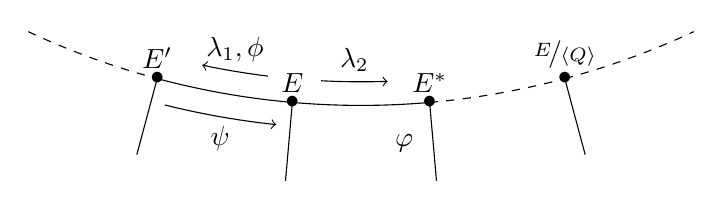
\begin{tikzpicture}[scale=1]
\coordinate (A) at (245:10);
\coordinate (B) at (255:10);
\coordinate (B') at (255:11);
\coordinate (B1) at (256:10.3);
\coordinate (C) at (265:10);
\coordinate (C') at (265:11);
\coordinate (D) at (275:10);
\coordinate (D') at (275:11);
\coordinate (E) at (285:10);
\coordinate (E') at (285:11);
\coordinate (F) at (295:10);
\coordinate (F') at (295:11);
\coordinate (G) at (305:10);
\coordinate (B2) at (258:9.7);
\coordinate (C1) at (266:10.3);
\coordinate (C2) at (267:9.7);
\coordinate (encre) at (273:10.5);
\draw (A) arc(245:255:10)[dashed];
\draw (B) arc(255:275:10);
\draw (D) arc(275:285:10)[dashed];
\draw (E) arc(285:295:10)[dashed];
\draw (B) node[above] {$E'$} node{$\bullet$};
\draw (C) node[above] {$E$} node{$\bullet$};
\draw (D) node[above] {$E^*$} node{$\bullet$};
\draw (E) node[above] {$\nicefrac{E}{\langle Q \rangle }$} node{$\bullet$};
\draw (encre) node {$\varphi$};
\draw (B)--(B');
\draw (C)--(C');
\draw (D)--(D');
\draw (E)--(E');
\draw (B1) arc(256:264:10.3) [->] node[below,midway] {$\psi$}; %flèche représentant \psi
\draw (B2) arc(258:263:9.7) [<-] node[above,midway] {$\lambda_1, \phi$}; %flèche représentant 
\draw (C2) arc(267:272:9.7) [->] node[above,midway] {$\lambda_2$}; %flèche représentant 
% \draw (C1) arc(266:284:10.3) [->];% node[below,midway,fill=white] {$\varphi $};

%\draw (260:10.75) node{}
%\draw (0,0) arc (245:255:10)[dashed] node[above] {$C$} node{$\bullet$} --(0:1.5);
%\draw (0,0) arc (245:255:10)[dashed] arc (255:265:10) node[above] {$E^i$} node{$\bullet$} --(0:1.5);
%\draw (-1,0) arc (245:255:10) node[above] {$C2$} node{$\bullet$} --(90:1)[color=yellow];
%\draw (-1,0) arc (245:255:10) node[above] {$C$} node{$\bullet$} --(310:1.5)[color=red];
%\draw (0,0) arc (245:255:10)[color=white] node[above] {$C$} node{$\bullet$} arc (255:265:10) node[above] {$E^i$} node{$\bullet$} arc (265:275:10) node[above] {$E$} node{$\bullet$} arc (275:285:10) node[above] {$F$} node{$\bullet$} arc (285:295:10) node[above] {$G$} node{$\bullet$} ; 
\end{tikzpicture}
\end{center}
\caption{ Example for the case $\ell=2$ } 
\end{figure}
\begin{algorithm}
\caption{\label{alg:horizontal}Computing a horizontal point of order~$ℓ^k$}
% Horizontalisation of $R$ following the $\lambda$ direction}
\begin{algorithmic}[1]
\REQUIRE $(P, Q)$: a diagonal basis of~$E[ℓ^{h+1}]$; $k$: an integer.\\
% $R$: a point of~$E$ of order $ℓ^k$ such that
% $ℓ^n R$~is horizontal of direction~$μ$ for some~$n ≤ k$.
\ENSURE $R$: a horizontal point of~$E[ℓ^k]$ with direction~$λ$.
% \ENSURE $E →^{ϕ_1} E_{1} … E_{n-1} →^{ϕ_n} E_n$:
% a chain of $n$ horizontal $ℓ$-isogenies of direction~$λ$;\\
% $(P_n,Q_n)$: a diagonal basis  of~$E_n[ℓ^{h+1}]$.
\STATE $E_0 \gets E$; $(P_0, Q_0) \gets (P, Q)$.
\FOR{$i = 1$ to~$k-1$}
\STATE $ϕ_i \gets $ isogeny with kernel~$ℓ^{h} P_{i-1}$
\STATE $Q_{i} \gets ϕ_i(Q_{i-1})$
\STATE $P' \gets ϕ_i(P_{i-1})/ℓ$.
\STATE Write~$π(P') = λ P' + b Q_i$ for~$b ∈ ℤ/ℓℤ$ and
let $P_{i} \gets P' - (b/μ) Q_i$.
\ENDFOR
\RETURN $R = \widehat{ϕ}_1 ∘ … ∘ \widehat{ϕ}_{k-1} ( ℓ^{-k+1} P_{k-1} )$.
% \RETURN $\{\widehat{ϕ}_1,..,\widehat{ϕ}_n\}, R_n, P_n$
\end{algorithmic}
\end{algorithm}
\begin{prop}
Algorithm~\ref{alg:horizontal} is correct and has a complexity of
% The computation complexity of algorithm \ref{alg:diagonal} is
%\begin{equation*}
%\begin{array}{ll}
%O\pa{\cout{M}(ℓ^k) · k · (k + \log q)}, &\text{if $ℓ = 2$;}\\
%O\pa{\cout{M}(ℓ^k) · ℓ^k · k^2 · \log ℓ · \log q
%  \;+\; k · \cout{F}(q, ℓ^k)}, &\text{if $ℓ ≠ 2$.}
%\end{array}
%\end{equation*}
\begin{equation*}
O(k(\mathsf{R}(k)+\mathsf{F}(k,0)))
\end{equation*}
\end{prop}
\begin{proof}
We check that at step~$i$ of the loop,
the points~$(P_i, Q_i)$ form a diagonal basis of~$E_i[ℓ^{h+1}]$,
and $ϕ_i$~has direction~$λ$.
The fact that $R$~is horizontal is then a consequence
of Proposition~\ref{prop:push-horizontal}.
% the point $ℓ^{n-i} R_i$ is horizontal with direction~$μ$,
% using Proposition~\ref{prop:push-horizontal} for the induction step.
% Since $ϕ_{i+1}$ is horizontal with direction~$λ$,
% according to Proposition~\ref{prop:push-horizontal},
% $ℓ^{n-i-1} R_{i+1} = ϕ_{i+1} (ℓ^{n-i-1} R_i)$ is also horizontal
% with direction~$μ$.
The complexity analysis %of Algorithm~\ref{alg:horizontal}
is exactly the same as for Algorithm~\ref{alg:diagonal}.
\end{proof}

% After execution of Algorithm~\ref{alg:horizontal},
% the point~$P_n$ is horizontal
% 
% In practice, we shall use Algorithm~\ref{alg:horizontal}
% in the case where~$R = Q_{k}$ as output from Algorithm~\ref{alg:diagonal}.
% In that case, since $Q_k$~is diagonal, $ℓ^{h} Q_k$~is horizontal,
% so that we may use~$n=h$.
One application of Algorithm~\ref{alg:diagonal} (with input~$k ← h+1$)
and two applications of Algorithm~\ref{alg:horizontal} allow us
to compute a horizontal basis of~$E[ℓ^k]$.
This could be done directly with Algorithm~\ref{alg:diagonal} instead,
but that would require computing in an extension
of degree up to~$ℓ^{k+h}$.

%Algorithme necessaire, surement pour enfoncer le clou...


%%%%%%%%%%%%%%%

\section{Interpolation step}
\label{sec:interpolation}
\subsection{Interpolating a polynomial on a field extension}

In this part, we consider the following problem. Consider a pair $(v,
w)$, with both $v$ and $w$ in $\F_{q^{\ell^m}}$, and $v$ of degree exactly
$\ell^m$ over $\F_q$. Our goal is to
compute polynomials $T$ and $L$ such that
\begin{itemize}
\item $T \in \F_q[x]$ is the minimal polynomial of $v$, so that $\deg(T) = \ell^m$;
\item $L$ is in $\F_q[x]$, of degree less than $\ell^m$, and $L(v)=w$.
\end{itemize}
In~\cite{df10}, De Feo gives a recursive algorithm for this task in the
context of Artin-Schreier extensions, which was inspired by earlier
work by Enge and Morain for solving equations by radicals~\cite{enge+morain03}.
In this paragraph, we adapt De Feo's algorithm to our context, in a straightforward manner. 
\todo{Say that we assume that $\ell-1$ divides $q$, and that we
use a cyclotomic-something tower.}



\begin{lem}\label{lemma:frob-ell} \todo{peut etre bouger cela ailleurs ou le mentionner dans la section 1}
  Let $a$ be in $\F_{q^{\ell^e}}$, and suppose that $\F_{q^{\ell^e}}$
  is represented as XXX. For any integer $v$, we can compute
  $a^{q^{\ell^v}}$ using $O(\ell^e)$ operations in $\F_q$, after a
  precomputation independent from $a$ that uses $O(\log(q))$
  operations in $\F_q$ and $\tilde{O}(\ell^e \log(q))$ bit operations.
\end{lem}
\begin{proof}
  This is a direct generalization of the case $\ell=2$ from~\cite{DoSc12}.
  Without loss of generality, we can assume that $v < e$; otherwise,
  the output is simply $a$ itself. By assumption, $a$ is written as
  $a =a_0 + a_1 x + \cdots + a_{\ell^e-1} x^{\ell^e-1}$, for some $x$
  that satisfies $x^{\ell^e}=c$, with $c$ in $\F_q$. 

  The first step, independently of $a$, is to compute
  $y=x^{q^{\ell^v}}$. Writing $q^{\ell^v} = u \ell^e + r$, with $r <
  \ell^e$, we see that $y$ is given by $c^{u \bmod (q-1)}x^r$, which
  can be computed in $O(\log(q))$ operations in $\F_q$ once $u \bmod
  (q-1)$ and $r$ are known.  To find $u \bmod (q-1)$ and $r$, first
  compute $q^{\ell^v}$ modulo $\ell^e(q-1)$ and take respectively the
  quotient and remainder in the division by $\ell^e$. This can all be
  using in boolean time quasi-linear in $\ell^e \log(q)$.

  Finally, once we know $y$, we compute $a(y)$; all powers $y^i$ we need
  are themselves monomials in $x$, and can be computed in time $O(\ell^e)$.
\end{proof}

De Feo's algorithm first computes $T$, starting from $T^{(0)}=x-v$.
For $i=0,\dots,m-1$, suppose we know a polynomial $T^{(i)}$ of degree
$\ell^i$ in $\F_{q^{\ell^{m-i}}}[x]$. Then, compute the polynomials
$T^{(i,j)}$ given by
$$T^{(i,j)}= \pi^{\ell^{j(m-i-1)}}\left (T^{(i)} \right)$$
for $0 \le j \le \ell-1$
and define 
$$T^{(i+1)}=\prod_{j=0}^{\ell-1} T^{(i,j)};$$ one easily sees that
$T^{(i)}$ is the minimal polynomial of $v$ over $\F_{q^{\ell^{m-i}}}$,
and in particular that $T^{(m)}=T$.  At step $i$, using
Lemma~\ref{lemma:frob-ell}, we see that computing a single Frobenius
takes $O(\ell^m)$ operations in $\F_q$, for a total of $O(\ell^{m+1})$
for all $\ell$ of them (together with a precomputation that costs
$O(\log(q))$ operations in $\F_q$ and $\tilde{O}(\ell^{m-i} \log(q))$
bit operations. Summing over all $i$, the total time for the
Frobeniuses is is $O(m \ell^m)$ operations in $\F_q$, plus a
precomputation that takes $O(m \log(q))$ operations in $\F_q$ and
$\tilde{O}(\ell^{m} \log(q))$ bit operations.

Deducing $T^{(i+1)}$ from the $T^{(i,j)}$'s can be done using
subproduct tree techniques, as in~\cite[Chapter~10]{vzGG}. 
%\todo{The following should go somewhere else.} We start
%by the following claim, which is Lemma~2.2 in~\cite{vzgathen+shoup92}.

%\begin{lem}\label{lemma:complexity_pol_mul} Let $\mu$ be a non-negative integer.
%  The cost of multiplying two polynomials of degree $n$ in
%  $\mathbb{F}_{q^{\ell^\mu}}[x] $ is $O(\mathsf{M}(\ell^\mu n))$ operations in
%  $\mathbb{F}_q$.
%\end{lem}


\begin{lem} \label{lemma:mul-pol}
  Let $R_1,\dots,R_s$ pairwise coprime polynomials in
  $\F_{q^{\ell^\mu}}[x]$, with sum of degree $t$. Then one can compute the
  polynomial $R=R_1 \cdots R_s$
  using $O(\mathsf{M}(\ell^\mu t) \log(s) )$ operations in $\F_q$.
\end{lem}
\begin{proof}
  The algorithm is well-known, see for
  instance~\cite[Lemma~10.4]{vzGG}; the analysis however has to be
  adapted to our context in order to derive the claimed cost bound.

  Following the previous lemma, let $c$ be such that we can multiply
  polynomials of degree $n$ in $\mathbb{F}_{q^{\ell^\mu}}[x] $ in at
  most $c M(\ell^\mu n)$ operations in $\F_q$. The multiplication
  algorithm we use involves $O(\log(s))$ steps. At each of them, we
  rely on several products of polynomials, the sum of which degrees is
  at most $n$.
  
  Consider a given step, say $i$, and let
  $(S_{i,1},U_{i,1}),\dots,(S_{i,t_i},U_{i,t_i})$ be the pairs of
  polynomials we have to multiply. Let $(\nu_{i,j},\eta_{i,j})$ be the
  degrees of $(S_{i,j},U_{i,j})$; in view of the discussion above, we
  see that multiplying these two polynomials takes at most $c
  \mathsf{M}(\ell^\mu (\nu_{i,j}+\eta_{i,j}))$ operations in
  $\F_q$. Summing over all $j$, and using the assumption that the sum
  of all $\nu_{i,j}+\eta_{i,j}$, for fixed $i$, is at most $n$, we
  conclude that the cost at step $i$ is at most $c \mathsf{M}(\ell^\mu
  n)$ operations in $\F_q$. Taking all steps into account, we finish
  the proof.
\end{proof}

Thus, we can compute $T^{(i)}$ using $O(\mathsf{M}(\ell^m)\log(\ell))$
operations in $\F_q$, and for all $T^{(i)}$'s, and in particular $T$,
the time becomes $O(\mathsf{M}(\ell^m)\log(\ell^m))$.

Next, we compute $T'(v)$. This is done by means of successive
Euclidean remainders, since $T'(v) = (((T' \bmod T^{(1)}) \bmod
T^{(2)}) \cdots \bmod T^{(m)})$.  At stage $i$, we have to compute 
the Euclidean division of polynomials of degree $O(\ell^{m-i})$ 
in $\F_{q^{\ell^i}}[x]$. Using Lemma~\ref{lemma:complexity_pol_mul},
and the fact that Euclidean division can be reduced to polynomial 
multiplication, we deduce that each division can be done in time
$O(\mathsf{M}(\ell^m)\log(\ell))$, for a total of 
$O(\mathsf{M}(\ell^m)\log(\ell^m))$ operations in~$\F_q$.

We can finally proceed with the interpolation itself. First, compute
$w' = w/T'(v)$ and let $L^{(0)}=w'$; this takes $O(\mathsf{M}(\ell^m)\log(\ell^m))$ operations in $\F_q$.
Next, for $i=0,\dots,m-1$, suppose we
know a polynomial $L^{(i)}$ in $\F_{q^{\ell^{m-i}}}[x]$
 of degree less than
$\ell^i$. We compute the polynomials $L^{(i,j)}$ given by
$$L^{(i,j)}= \pi^{\ell^{j(m-i-1)}}\left (L^{(i)} \right),$$
for $0 \le j \le \ell-1$, 
and 
$$L^{(i+1)} = \sum_{0 \le j \le \ell-1} L^{(i,j)} T^{(i,0)} \cdots
T^{(i,j-1)} T^{(i,j+1)} \cdots T^{(i,\ell-1)}.$$ As proved
in~\cite{df10}, $L^{(m)}$ is the polynomial $L$ we are looking for.
The cost induced by the recombination above is of the same order as
that seen previously for the computation giving
$T^{(i+1)}$. Altogether, the total is $O(\mathsf{M}(\ell^m)
\log(\ell^m))$ operations in $\F_q$, plus a precomputation that takes
$O(m \log(q))$ operations in $\F_q$ and $\tilde{O}(\ell^{m} \log(q))$
bit operations. \todo{don't call this a precomputation, and handle it better.}
\todo{write a proper proposition}

\subsection{Taking all orbits into account}
\todo{du coup a deplacer vers le 5}
In this section we work with the points of order $\ell^k$ on two input
curves $E,E'$ as in Problem~\ref{prob:isogeny-problem}, that lie on
the cyclic crater of a volcano of $\ell$-isogenies (in all this
section, $k$ is fixed).
As input, we are given horizontal bases $(P,Q)$ of $E[\ell^k]$ and
$(P',Q')$ of $E'[\ell^k]$ as computed in
Section~\ref{sec:acti-frob-endm}, together with two coefficients $(a,b)
\in \left(\mathbb{Z}/\ell^k \mathbb{Z} \right)^*$. For the discussion below,
let $S$ and $S'$ denote the set of abscissae of points of order
$\ell^k$ on respectively $E$ and $E'$.

The algorithm in this section computes two polynomials. The first of
them is $T(x)$, which is the squarefree monic polynomial whose roots
are the elements in $S$; in particular, it does not depend on
$E'$. More crucially, we also compute an interpolation polynomial
$L(x)$ that maps $S$ to a permutation of $S'$ induced by the mapping
$P \mapsto aP'$ and $Q \mapsto bQ'$.

Precisely, this means that we ask that $L(x(cP+dQ))=x(caP'+dbQ')$
holds for all pairs $(c,d) \in (\mathbb{Z}/\ell^k\mathbb{Z})^2$ for
which either $c$ or $d$ is coprime with $\ell$, in which case $cP+dQ$
and $acP'+dbQ'$ have order $\ell^k$; here, $x(P)$ denotes the abscissa
of a point $P$.  
\newline
\begin{prop}
The points of order $\ell^k$ of $E$ are of order $\ell^{\beta+k}=o_j  \leqslant o_i \leqslant o_0=  \ell^{\alpha+k} $ for the Frobenius action according to the structure of $E[\ell^\infty](\F_k)$.
\newline
Moreover the sets of representatives of points of order $o_i$ are of size $\frac{\ell^2k-2}{\ell^{\alpha+k}}$ for $i \in \{1,..,j-1\}$ and of size $\frac{\ell^{2k-1}}{\ell^{\alpha+k}}$ for $i=0$ and $i=j$.
\end{prop}
The computations of representants of the different orbits is done working only with indexes in $(\mathbb{Z}/\ell^k \mathbb{Z}^*)^2$ of the basis $(P,Q)$. Once we have the indexes we compute the corresponding points. Since there is $O(\ell^k)$ points of different orbits we can state the following result:

\begin{prop}\todo{a verifier plus en detail..., voir si on peut pas se servir de la proposition de Jerome}
The cost of computings the different representatives of orbits is $O(\ell^kM(\ell^k)k \log(\ell))$.
\end{prop}

\begin{proof}
\todo{ce qui suit n est pas une preuve mais une intuition}
As we consider a set of $\ell^{2k-2}\frac{\ell^2-1}{\ell^2}$ points of order $\ell^k$ with orbits of size going to $\ell^{k-\alpha}$ to $\ell^{k-\beta}$ then will have at most $\ell^{k-2+\beta}\frac{\ell^2-1}{\ell^2}$ representants of different orbits.
\end{proof}

Now we can apply the results of the preceding subsection to compute for each representative of orbits of order $o_i$ their interpolation polynomial associated in $O(\log(o_i)M(o_i))$ operations on $\mathbb{F}_q$ for $i \in \{0,..,j\}$. We can then recombine all those results using Chinese Remainder Theorem. We can notice also that the modulus for the Chinese Remainder Theorem do not depend of the choices of the coefficients $(a,b) \in (\mathbb{Z}/\ell^k \mathbb{Z}^*)^2$, thus we can use this to speed up the next occurrences of the CRT by doing precomputation for the inverse of the modulus in the CRT, we will state two complexity analysis for the CRT .

\begin{prop}
The cost of the C.R.T. applied on all the different orbits for the first occurence is of $O(M(\ell^{2k})\log(\ell^{2k}))$ operations in $\mathbb{F}_q$. For the next occurences the cost is of $O(M(\ell^{2k})\log(\ell^{k}))$ operations in $\mathbb{F}_q$.
\end{prop}

\begin{proof}
The first assertion comes from the fact that there is $\ell^{2k-2}\frac{\ell^2-1}{\ell^2}$ points of order $\ell^k$ and we work with polynomials in $\mathbb{F}_q[x]$. The second one comes from the fact that we have $O(\ell^k)$ representatives of orbits and we do only multiplication and additions on the polynomials associated to the orbits, we conclude by lemma \ref{lemma:mul-pol}
\end{proof}

\todo{Do it by splitting the set of $\ell^k$ torsion into orbits for
  the Frobenius. Each orbit can be handled in quasi-linear time using
  the previous subsection, and the recombination is just Chinese
  remaindering over $\F_q$, so we should be good.}

\todo{Make sure that computing one representative per orbit is not too
  expensive.}

\section{The complete algorithm}
\label{sec:complete-algorithm}
%%%%%%%%%%%%%%%
\subsection{Finding a suitable $ℓ$-volcano}
\label{sub:shape-volcano}

Our algorithm uses an Elkies prime~$ℓ$.
According to Chebotarev's density theorem,
\todo{apparemment selon qu'on transcrit depuis le russe ou l'ukrainien
son nom change, je voudrais ne pas trop troller le referee si possible}
the density of primes~$ℓ$ such that~$(d_K/ℓ) = +1$ is asymptotically~$1/2$,
so that we need only try a $O(1)$ number of primes~$ℓ$.
Since~$d_K$ is not assumed to be known yet,
we need to be able to compute the shape of the crater,
as well the shortest $ℓ$-isogeny chain from~$E$ to the crater.

\todo{Eventually explicit the complexity of computing a shape of the volcano i.e. $\mathcal{F}(\ell)$}
% One crucial point before starting to use methods described above is to determine if the input curves of problem \ref{prob:isogeny-problem} are located on a cylic crater of a volcano and if it is not the case compute a the shortest chain of $\ell$-isogeny to a curve on the crater. 
%   \newline
  For $\ell \neq 2$ after determining a chain of $\ell$-isogeny to a curve on the crater we determine which kind of crater the curve is located on by looking for  the length of $(\ell+1)$ descending chain of $\ell$-isogenies on the volcano, all those methods are described in \cite{volcano}. If there is two paths of length greater than the others then the crater is cyclic, if not the crater is not cyclic. This is done in a complexity of $O( ( \frac{\log(q)}{\log(\ell})^2 \mathcal{F}(\ell) )$, with $h=O(( \frac{\log(q)}{\log(\ell}))$ the height of the volcano (not known a priori) and $\mathcal{F}(\ell)$ the cost of computing three roots of a $\ell$ modular polynomial of $O(\ell^2+M(\ell)\log(q))$. We can also mention methods used in \cite{IonicaJ10} which are done in a complexity of $O(h(\ell^3+\ell \mathsf{M}(\ell) \log(q)))=O(( \frac{\log(q)}{\log(\ell})(\ell^3+\ell \mathsf{M}(\ell) \log(q)))$ and take advantage of the structure of the $\ell$ torsion when it is linked with the level in volcano with pairings that determine ascending or horizontal $\ell$-isogenies. %when the curve is not located over a stability level.
\newline 
For $\ell=2$ we can use methods like in \cite{MiretMRV05}. The height and the shape of the volcano can be computed with a complexity of $O(\log^6(q))$ which computes an ascending path and can determine the shape of the crater by taking advantage of the torsion structure when it is linked with the level in volcano otherwise it uses methods similar to \cite{volcano}.
 %c est exactement ce qui est fait dans ce papier...
  
\subsection{Lifting the problem to a cyclic crater}

If the two input curves~$E$, $E'$ of our algorithm
belong to cyclic $ℓ$-isogenies volcanos but not to their crater,
then by Proposition~\ref{prop:parallel},
their depth below the craters is the same.
Using the methods of~\ref{sub:shape-volcano},
we can compute the shortest path of $ℓ$-isogenies~$α: E → E_{\max}$,
$α': E' → E'_{\max}$ linking the curves~$E, E'$ to the craters.
By Proposition~\ref{prop:parallel} (iii),
the curves~$E_{\max}$ and~$E'_{\max}$ are again $r$-isogenous;
we can use our algorithm to compute such an isogeny~$ψ_{\max}$.
Then $ψ = (α')^{-1} ∘ ψ_{\max} ∘ α$ is the required $r$-isogeny.

 \subsection{Curves which are on the cyclic crater}
  The previous sections \ref{sec:acti-frob-endm}, \ref{sec:interpolation} describe steps of the algorithm for curves located on the crater of cyclic volcano (Elkies) thus for this subsection we consider two input curves at the problem \ref{prob:isogeny-problem} in this situation. 
\newline
\todo{complete the complexity}
 First we compute $k$ such that $\frac{3}{2}\ell^{2k-2}>r$, then we compute a basis of the $\ell$ torsion solving a division polynomial of degree $\ell^2$, thus we have a complexity of $O(M(l)\log(\ell) \ell^5 \log(\ell^2) \log(q))$, using Cantor-Zassenhauss in $F_1$ with $d$ the order of $q$ in $\mathbb{Z}/\ell\mathbb{Z}^*$.%Cantor Zassenhauss dans F_1
 Then we use algorithm \ref{alg:diagonal} to obtain a diagonal basis $(P,Q)$ of the $\ell^k$ torsion with a complexity of $O(k(\mathsf{R}(k)+\mathsf{F}(k,0)))$. Using notations of algorithm \ref{alg:horizontal} we apply this algorithm to $(P,Q,Q)$, we get then $(P_{k-h},Q_{k-h})$ a diagonal basis of $E_{k-h}[\ell^k]$ and a chain of $\ell$ isogeny of direction $\mu$, we then apply successively the isogenies of the chain on $P_{k-h}$ and we get in the end a horizontal point $P$ of $E$ of direction $\lambda$. We use a similar method to get $Q$ an horizontal point of $E$ of direction $\mu$. Thus the cost of computing an horizontal basis is the same as algorithm \ref{alg:horizontal}: $O(k(\mathsf{R}(k)+\mathsf{F}(k,0)))$.  Now we can describe the entire algorithm for elliptic curves located on the cyclic crater of a volcano.
\newline  
  As like the Couveignes' algorithm we proceed in 3 steps to solve problem \ref{prob:isogeny-problem}:
 \begin{enumerate}
\item Compute horizontal basis $P,Q$ and $P',Q'$ of
  $E[\ell^k]$ and $E'[\ell^k]$ respectively, for $\frac{3}{2}\ell^{2k-2} > 4r$ \todo{preciser cette borne} ;
\item\label{alg:modif-couveignes:interp} Choose $(a,b) \in (\mathbb{Z}/\ell^k\mathbb{Z}^*)^2$ and compute the interpolation
  polynomial $L$ \todo{(verify that notation is consistent
    with Sec.4)} sending $x(P)$ to $x(aP')$ and $x(Q)$ to $x(bQ')$, and the abscissas of
  their scalar multiples of order $\ell^k$ accordingly;
\item\label{alg:modif-couveignes:rational} Deduce a rational fraction
  congruent to $L$ modulo $T$, and verify that it
  defines an isogeny of degree $r$. If it does, return it, otherwise
  replace $P',Q'$ with an other horizontal basis of $E'[\ell^k]$ and go back to
  Step~\ref{alg:orig-couveignes:interp}.
\end{enumerate} 

\begin{prop}
The complexity of solving problem \ref{prob:isogeny-problem} for two elliptic curves located on a cyclic crater of volcano of $\ell$ isogeny is for $\ell=2$ of $O(rM(r)\log(r))$ in $\mathbb{F}_q$ and for $\ell \neq 2$ of $O(rM(r)\log(r)+r^2F(q,\ell^k))$ in $\mathbb{F}_q$.
\end{prop}

\begin{proof}%refaire ça avec les notations de Luca
The cost of computing horizontal basis is for $\ell=2$ of $O((\log(r)^2+\log(r)\log(q))M(\sqrt{r}))$ in $\mathbb{F}_q$, for $\ell \neq 2$ it is of $O(\sqrt{r}\log(q)M(\sqrt{r})\log(r)^2 \log(\ell)^{-1}+kF(q,\ell^k))$ in $\mathbb{F}_q$.
The cost of computing an interpolation polynomial is for $\ell=2$ of $O(M(r)\log(r))$, for $\ell \neq 2$ it is of $O(M(r)\log(r)+rF(q,\ell^k))$ . The rational reconstruction is done in $O(M(r)\log(r))$ operations in $\mathbb{F}_q$. In average we have to repeat this step $O(\ell^{2k})=O(r)$ times. 
Thus we have a total complexity for $\ell=2$ of  $O(rM(r)\log(r))$ in $\mathbb{F}_q$ and for $\ell \neq 2$ of $O(rM(r)\log(r)+r^2F(q,\ell^k))$ in $\mathbb{F}_q$.
\end{proof}
  
\section{Experimental results}
\label{sec:implem}

\todo{Describe implementation and show benchmarks. Possibly compare
  with Lercier-Sirvent (Luca has an implementation somewhere).}

\begin{acknowledgements}
  We thank many people.
\end{acknowledgements}

\bibliographystyle{alpha}
\bibliography{refs}


\appendix
\section{Isogenies and the Tate module}
\label{ap:Tate}
We recall here a few results about $ℓ^n$-isogenies
and the $ℓ$-adic Tate module.

The isogeny determined by a point~$P$ of order~$ℓ^n$ only depends on
the subgroup~$\chev{P}$ generated by~$P$ in~$E[ℓ^n]$.
Equivalently, this subgroup defines a point in
the projective space of~$E[ℓ^n]$,
which is a projective line over~$ℤ/ℓ^n ℤ$.

There exists a canonical bijection~\cite[II.1.1]{SL2} between
this projective line and
the set of lattices of index~$ℓ^n$ in the $ℤ_ℓ$-module $T_ℓ(E)$:
it maps a line~$\chev{P}$ to the lattice~$Λ_P = \chev{P} + ℓ^n T_ℓ(E)$.
This lattice is also the preimage by the isogeny~$ϕ_P: E → E_P$
of the lattice~$ℓ^n T_ℓ(E_P)$.

\medbreak
If a basis~$(R, S)$ of~$E[ℓ^n]$ is fixed and~$P = a R + b S$,
then the lattice~$Λ_P$ is generated by the columns of the matrix
$L_P = \smat{ℓ^n & 0 & a\\0 & ℓ^n & b}$.
Write~$b = ℓ^m b'$ with~$ℓ ∤b'$; the Hermite normal form of~$L_P$
is $M_P = \smat{ℓ^{n-m} & a/b' \\ 0 & ℓ^m}$,
and its columns also generate the lattice~$Λ_P$.
We check that $M_P$ has determinant~$ℓ^n$.
Since $Λ_P = ϕ_P^{-1} (ℓ^n T_{ℓ} (E_P))$,
there exist bases of~$T_ℓ(E), T_ℓ(E')$
in which $Φ_P$ has the matrix~$ℓ^n M_P^{-1}$.
Therefore, in that basis of~$T_ℓ(E_P)$,
the matrix of~$π|T_ℓ(E_P)$ is $M_P^{-1} · π · M_P^{}$.

\section{Division of a point by~$\ell$}
\label{ap:division}

We write~$Q ← P/ℓ$ for the computation of a preimage of~$P$
by multiplication by~$ℓ$.
The obvious way to compute~$P/ℓ$ would be to use the $ℓ$-division polynomial.
However, this polynomial has a degree~$O(ℓ^2)$.
Instead, we factor the multiplication-by-$ℓ$ map
as a product of an $ℓ$-isogeny and its dual.
This brings the polynomial degree down to~$O(ℓ)$.
According to subsection~\ref{sub:towers},
the cost of the $P/ℓ$ operation is therefore $\mathsf{R} (k)$.
%\begin{equation}\label{eq:div-by-l}
%O \pa{\cout{M}(ℓ^k) \,· \,\left\lbrace\begin{array}{ll}
%(k + \log q) & \text{if $ℓ = 2$,} \\
%(ℓ^k · k · \log ℓ · \log q) & \text{if $ℓ ≠ 2$.}
%\end{array}\right\rbrace}.
%\end{equation}
% \begin{equation}\label{eq:div-by-l}
% \mathsf{R}(k)
% \end{equation}

\begin{algorithm}
\caption{\label{ldivision}Compute the preimage of $Q$ by the multiplication by $\ell$.}
\begin{algorithmic}[1]
\REQUIRE  $(P_1,P_2)$ a basis of $E[\ell]$;\\
$Q$: a point on $E$ such that there exist a $\ell$ division point of $Q$.
\ENSURE $Q_1$: a point on $E$ such that $\ell Q_1 = Q$.
%\STATE compute $ (P_1,P_2)$ a basis of $ E[\ell]$
\STATE $\phi_1$ $\leftarrow$ the isogeny with kernel~$P_1$.
\STATE $\phi_2$ $\leftarrow$ the isogeny with kernel~$\phi_1(P_2)$.
\STATE $Q_2 \leftarrow$ preimage of $Q$ by $\phi_2$
\STATE $Q_1 \leftarrow$ preimage of $Q_2$ by $\phi_1$
\RETURN $Q_1$
\end{algorithmic}
\end{algorithm}


\end{document}
%  LocalWords:  isogeny morphisms Isogenies isogenies isogenous
%  LocalWords:  cardinality bijection Couveignes automorphism

% vim: ts=2:
%  LocalWords:  Frobenius endomorphism
